\subsection{Neural Nets}

% Derivation from biology {{{
\subsubsection{Derivation from biology}
\label{ss_nn_derivation_from_biology}

"Neural networks are an attempt to model the insights
gained in brain research on the interaction between nerve
cells (neurons) and connections (synapses)".\cite{ct_math}

Here, an artificial neuron mimics the functioning of a
nerve cell . A biological nerve cell is connected to other
nerve cells via synapses. At these connections, stimuli are
transmitted by means of chemical messengers
(neurotransmitters) and converted into an electrical signal
within the nerve cell.

The synapses of a nerve cell are located at so-called
dendrites (branches), from which the transmitted stimuli
are transmitted to the soma (cell body). It does matter how
far the synapse is from the soma. The closer a synapse is
to the soma, the stronger the stimulus transmission.\cite{%
bio,ct_math}

In addition, it should be the case that multiple synapses
stimuli at the same time which adds incoming stimuli within
the nerve cell.\cite{bio} If the stimulus transmitted
exceeds a threshold within the cell, then an action
potential is triggered and the cell forwards the signal to
other cells, which in turn are connected via synapses to
the stimulating transmitting cell. Nerve cells form
associations in the human brain, which develop the ability
to recognize complex structures. Artificial neural networks
are an attempt to imitate these associations of nerve
cells.\cite{ct_math}
% }}}

% Structure of an artificial neuron {{{
\subsubsection{Structure of an artificial neuron}

\begin{figure}[H]
	\begin{center}
	\begin{tikzpicture}[%
    dot/.style={circle,draw,thick,fill=green!20}
  ]
		\node at (5,0) (out) {};
		\node at (0,0) [dot] (neuron) {$t=\sum_{i=1}^{n}{w_ix_i}$}
			edge[->,thick] node[above]{$\varphi(t-\theta)$} (out);
		\node at (-4,4) [dot] {$x_1$}
			edge[->,thick] (neuron);
		\node at (-4,2) [dot] {$x_2$}
			edge[->,thick] (neuron);
		\node at (-4,0) [dot] {$x_3$}
			edge[->,thick] (neuron);
		\node at (-4,-4) [dot] {$x_n$}
			edge[->,thick] (neuron);
		\node at (-4,-1.5) [tokens=1] {};
		\node at (-4,-2) [tokens=1] {};
		\node at (-4,-2.5) [tokens=1] {};
	\end{tikzpicture}
	\end{center}
	\caption{Scheme of an artificial neuron}
	\label{fig_neuron}
\end{figure}



From chapter \ref{ss_nn_derivation_from_biology}, the
components and functioning of an artificial neuron can be
derived.
\newline\newline
In an artificial neuron the following happens:

\begin{enumerate}

  \item An artificial neuron is connected to other neurons
        or the direct value input via input connections,
        which are supposed to represent the synapses of the
        nerve cell (described in Figure \ref{fig_neuron}
        with $x_i$). These inputs can be discreet or
        continuous.\cite{nne_beck}

        If the data comes from other neurons, the weighting
        of the connection is additionally transferred to
        the value $\omega_i$ . Each connection of a neuron
        has an individual weighting. The greater the value
        of this weighting, the more important the
        transmitted value $x_i$ for the network output.

  \item The value and weight of each input connection is
        added by the transfer function $\sum_{i=1}^{n}w_ix_i$
        to calculate the net input value $t$.


  \item Every artificial neuron, like a nerve cell, has a
        threshold. An artificial neuron is a value
        $\theta$. The threshold $\theta$ is subtracted from
        the net input value $t$ to determine the activation
        potential of the neuron.

        The threshold can also be represented by the bias.
        The bias is a further input, which transmits the
        constant value 1 and as weighting the value
        $b=-\theta$.

        	\begin{figure}[H]
		\begin{center}
			\begin{tikzpicture}[dot/.style={circle,draw,thick,fill=green!20,minimum size=1cm}]
				\node at (5,0) (out) {};
				\node at (0,0) [dot] (neuron) {$t=\sum_{i=1}^{n}{w_ix_i}+b$}
					edge[->,thick] node[above]{$\varphi(t)$} (out);
				\node at (-4,4) [dot] {$1$}
					edge[->,thick] node[anchor=south west]{$b=-\theta$} (neuron);
				\node at (-4,2) [dot] {$x_1$}
					edge[->,thick] (neuron);
				\node at (-4,0) [dot] {$x_2$}
					edge[->,thick] (neuron);
				\node at (-4,-4) [dot] {$x_n$}
					edge[->,thick] (neuron);
				\node at (-4,-1.5) [tokens=1] {};
				\node at (-4,-2) [tokens=1] {};
				\node at (-4,-2.5) [tokens=1] {};
			\end{tikzpicture}
		\end{center}
    \caption{An artificial neuron with bias}
    %\label{bn}
	\end{figure}



  \item The determined value of $t-\theta$ is used as an
        input in the activation function to determine the
        output of the neuron.

        From this process, the basic elements of a neuron
        can be determined:

        \begin{itemize}

          \item Weighting

          \item Threshold

          \item Transfer function

          \item Activation function

        \end{itemize}

\end{enumerate}
% }}}

% Construction of a neural network {{{
\subsubsection{Construction of a neural network}

\begin{figure}[H]
  \begin{center}
	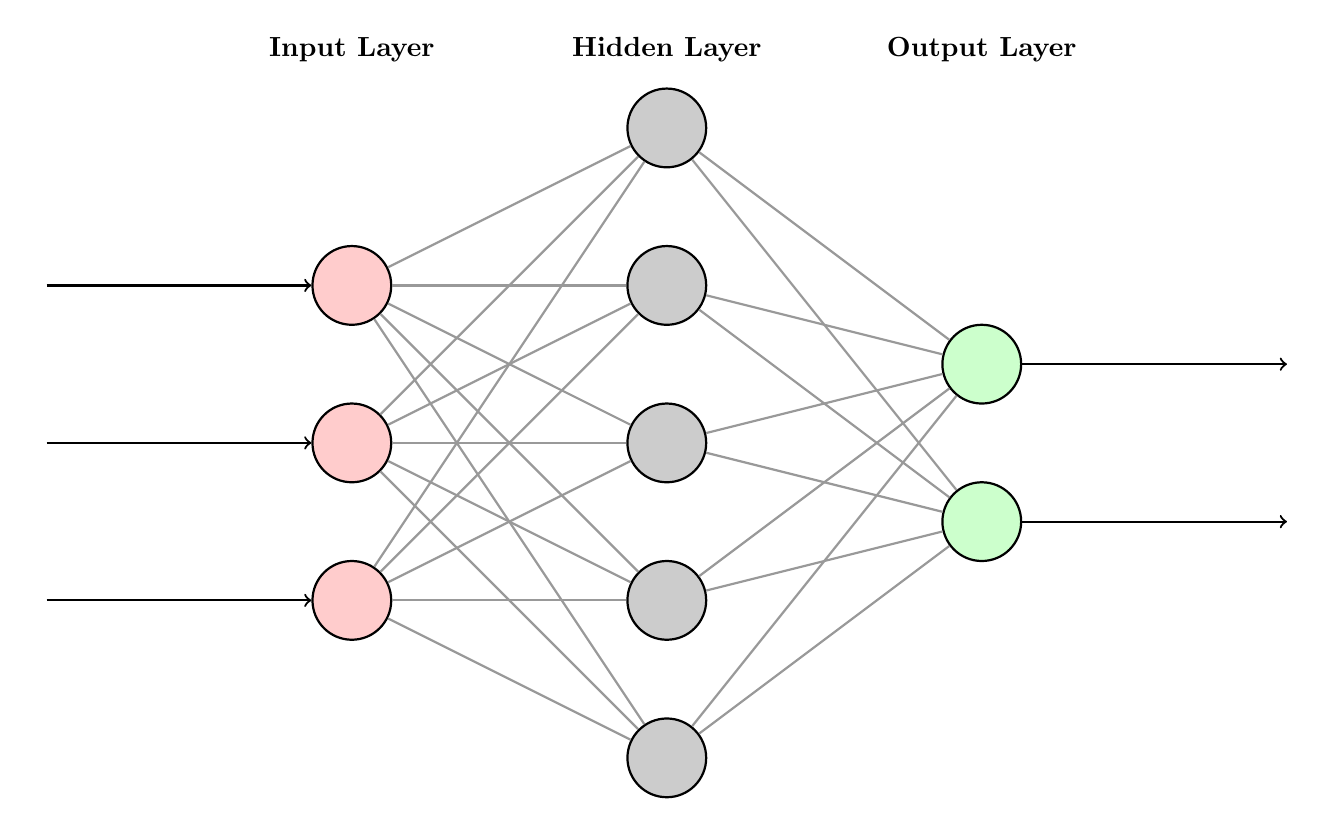
\begin{tikzpicture}[%
    dot/.style={circle,draw,thick,minimum size = 1cm}
  ]
		\node at(-4,5) {\textbf{Input Layer}};
		\node at(0,5) {\textbf{Hidden Layer}};
		\node at(4,5) {\textbf{Output Layer}};

		\node at(8,1) (oo1) {};
		\node at(8,-1) (oo2) {};

		\node at (4,1) [dot,fill=green!20] (o1) {}
			edge[->,thick] (oo1);
		\node at (4,-1) [dot,fill=green!20] (o2) {}
			edge[->,thick] (oo2);

		\node at (0,4) [dot,fill=black!20] (h1) {}
			edge[thick,black!40] (o1)
			edge[thick,black!40] (o2);
		\node at (0,2) [dot,fill=black!20] (h2) {}
			edge[thick,black!40] (o1)
			edge[thick,black!40] (o2);
		\node at (0,0) [dot,fill=black!20] (h3) {}
			edge[thick,black!40] (o1)
			edge[thick,black!40] (o2);
		\node at (0,-2) [dot,fill=black!20] (h4) {}
			edge[thick,black!40] (o1)
			edge[thick,black!40] (o2);
		\node at (0,-4) [dot,fill=black!20] (h5) {}
			edge[thick,black!40] (o1)
			edge[thick,black!40] (o2);

		\node at (-4,2) [dot,fill=red!20] (i1) {}
			edge[thick,black!40] (h1)
			edge[thick,black!40] (h2)
			edge[thick,black!40] (h3)
			edge[thick,black!40] (h4)
			edge[thick,black!40] (h5);
		\node at (-4,0) [dot,fill=red!20] (i2) {}
			edge[thick,black!40] (h1)
			edge[thick,black!40] (h2)
			edge[thick,black!40] (h3)
			edge[thick,black!40] (h4)
			edge[thick,black!40] (h5);
		\node at (-4,-2) [dot,fill=red!20] (i3) {}
			edge[thick,black!40] (h1)
			edge[thick,black!40] (h2)
			edge[thick,black!40] (h3)
			edge[thick,black!40] (h4)
			edge[thick,black!40] (h5);

		\node at(-8,2) (ii1) {}
			edge[->,thick] (i1);
		\node at(-8,0) (ii2) {}
			edge[->,thick] (i2);
		\node at(-8,-2) (ii3) {}
			edge[->,thick] (i3);
	\end{tikzpicture}
  \end{center}
  \caption{Neural network with hidden layer}
  %\label{snn}
\end{figure}


% }}}
